\let\negmedspace\undefined
\let\negthickspace\undefined
\documentclass[journal]{IEEEtran}
\usepackage[a5paper, margin=10mm, onecolumn]{geometry}
%\usepackage{lmodern} % Ensure lmodern is loaded for pdflatex
\usepackage{tfrupee} % Include tfrupee package

\setlength{\headheight}{1cm} % Set the height of the header box
\setlength{\headsep}{0mm}     % Set the distance between the header box and the top of the text

\usepackage{gvv-book}
\usepackage{gvv}
\usepackage{cite}
\usepackage{amsmath,amssymb,amsfonts,amsthm}
\usepackage{algorithmic}
\usepackage{graphicx}
\usepackage{textcomp}
\usepackage{xcolor}
\usepackage{txfonts}
\usepackage{listings}
\usepackage{enumitem}
\usepackage{mathtools}
\usepackage{gensymb}
\usepackage{comment}
\usepackage[breaklinks=true]{hyperref}
\usepackage{tkz-euclide} 
\usepackage{listings}
% \usepackage{gvv}                                        
\def\inputGnumericTable{}                                 
\usepackage[latin1]{inputenc}                                
\usepackage{color}                                            
\usepackage{array}                                            
\usepackage{longtable}                                       
\usepackage{calc}                                             
\usepackage{multirow}                                         
\usepackage{hhline}                                           
\usepackage{ifthen}                                           
\usepackage{lscape}
\begin{document}
\bibliographystyle{IEEEtran}
\title{1.4.9.h}
\author{EE24BTECH11007 - Arnav Makarand Yadnopavit}
{\let\newpage\relax\maketitle}
\renewcommand{\thefigure}{\theenumi}
\renewcommand{\thetable}{\theenumi}
\setlength{\intextsep}{10pt} % Space between text and floats
\numberwithin{equation}{enumi}
\numberwithin{figure}{enumi}
\renewcommand{\thetable}{\theenumi}
Question:\\
Find the coordinates of the points which trisect the line segment joining the points
$\vec{P}$ \brak{4,2,-6} and $\vec{Q}$ \brak{10,-16,6}.\\
\solution
\begin{table}[h]
    \centering
    \begin{tabular}{|m{5em}|m{10em}|}
    \hline
    \textbf{Point} &\textbf{Coordinates} \\
    \hline
         $\vec{P}$ & \brak{4,2,-6} \\
    \hline
        $\vec{Q}$ & \brak{10,-16,6} \\
    \hline
\end{tabular}
    \caption{Given Values}
    \label{tab:1}
\end{table}
Given\\
Let $\vec{R}$ and $\vec{S}$ trisect $\vec{P}$ and $\vec{Q}$\\
Using Section Formula
\begin{align}
\vec{R}=\frac{1}{\frac{1}{2}+1}\brak{\frac{1}{2}\myvec{4\\2\\-6}+\myvec{10\\-16\\6}}\\
\vec{R}=\myvec{8\\-10\\2}\\
\vec{S}=\frac{1}{\frac{2}{1}+1}\brak{\frac{2}{1}\myvec{4\\2\\-6}+\myvec{10\\-16\\6}}\\
\vec{S}=\myvec{6\\-4\\-2}
\end{align}
\begin{figure}[h]
    \centering
    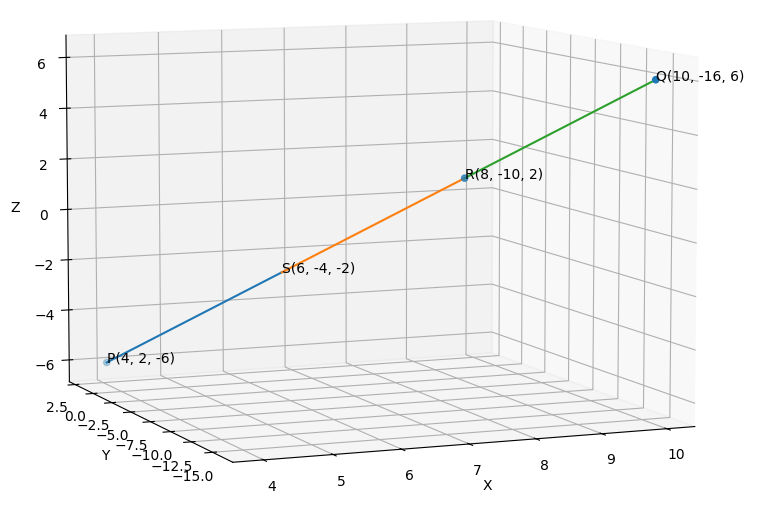
\includegraphics[width=\columnwidth]{figs/fig.png}
    \caption{Plot of $\vec{P}$,$\vec{Q}$,$\vec{R}$,$\vec{S}$}
 \end{figure}
\end{document}
